\documentclass[10pt,a4paper,oneside,openany]{book}
\usepackage{stc-common}
\geometry{margin=22mm,headheight=15pt,footskip=11mm}
\addbibresource{bibliography.bib}
\addbibresource{source-registry.bib}

\hypersetup{
  pdftitle={Sleep-Time Compute Conference Appendix},
  pdfauthor={Samsung SAIT Neural Memory Study},
  pdfsubject={Evidence chronology, scaling derivations, infrastructure, benchmark, and claim ledger}
}

\title{Sleep-Time Compute\\Conference Appendix}
\author{Samsung SAIT Neural Memory Study}
\date{Source freeze: 2026-08-05}

\begin{document}
\frontmatter
\maketitle
\chapter*{Appendix scope}
\addcontentsline{toc}{chapter}{Appendix scope}
이 부록은 conference main의 page budget 때문에 생략한 evidence chronology, evidence-maturity audit,
scaling derivation, infrastructure transaction, benchmark design, negative evidence와 canonical public claim
ledger를 보존한다. 각 장은 Full Study와 동일한 frozen source/figure ID를 사용한다.
During the preparation of this work the authors used Codex GPT-5.6 for evidence synthesis, LaTeX drafting,
and artifact QA. All content was reviewed and edited by the authors, who take full responsibility for the
accuracy and integrity of the work.
\tableofcontents

\mainmatter
\chapter{계보: biological replay에서 multi-rate neural memory까지}
\label{STC-S05}

Sleep-time compute는 2026년에 갑자기 생긴 단일 논문 계열이 아니다. Fast/slow learning theory,
continual learning, generative replay, external agent memory, test-time neural memory, asynchronous
memory agents가 서로 다른 문제를 풀다가 하나의 lifecycle로 수렴한다.

\begin{figure}[htbp]
  \centering
  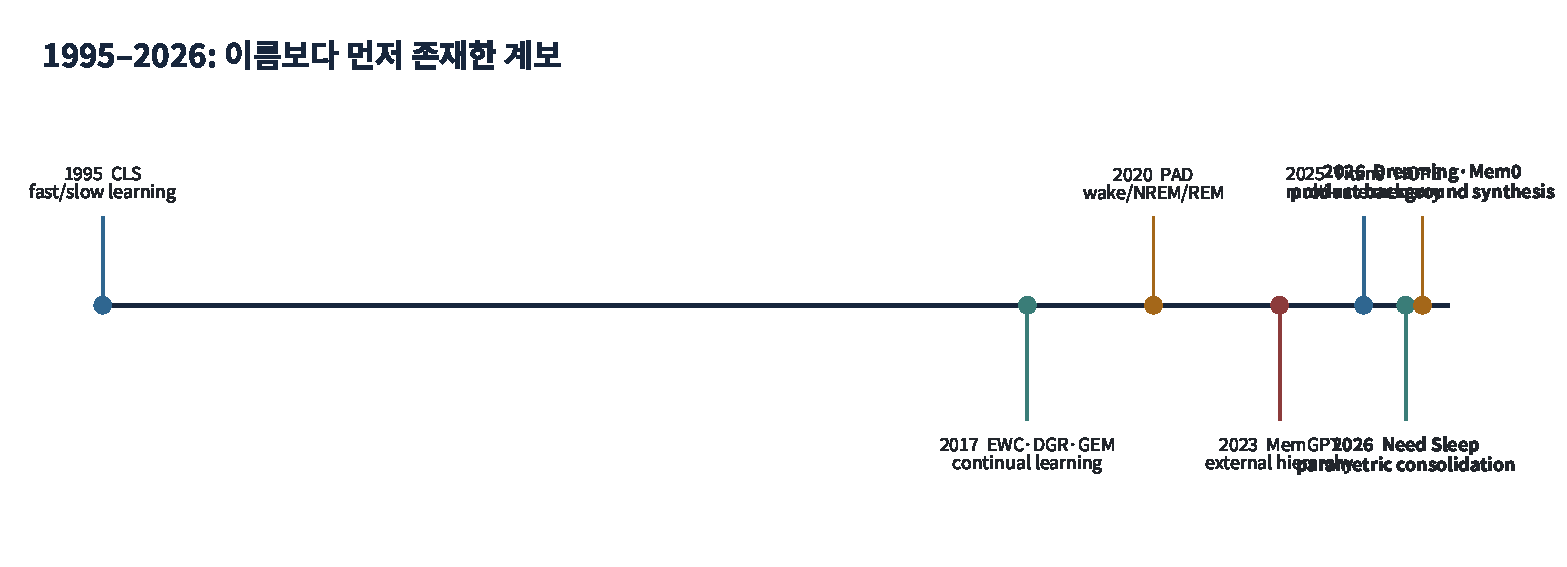
\includegraphics[width=0.98\textwidth]{figures/stc-f003.pdf}
  \caption{1995–2026 evidence chronology. 연도는 공개 source의 최초 publication/release 기준이며,
  같은 시기의 방법이 동일 maturity라는 뜻은 아니다.}
  \stcfigure{STC-F003}
  \figsource{Original synthesis; SRC-STC-0001--SRC-STC-0063}{1995 CLS에서 2017 continual learning, 2020 PAD, 2023 MemGPT, 2025 Titans/HOPE, 2026 parametric sleep과 product dreaming으로 이어지는 시간축.}
  \label{fig:stc-chronology}
\end{figure}

\section{1995: complementary learning systems}

CLS는 hippocampus의 빠른 episodic acquisition과 neocortex의 느린 interleaved learning을 분리했다
\parencite{srcstc0001}. 이 관점이 제공하는 basis는 ``새 기억을 빠르게 받는 store''와 ``기존 구조를
보존하며 천천히 통합하는 learner''를 한 update rule로 강제하지 않는다는 점이다. 오늘의 system으로
번역하면 wake log/episodic memory와 sleep consolidation model의 역할 분리다.

그러나 biology에서 production architecture를 곧바로 도출할 수는 없다. Biological model은 user
scope, exact delete, source attribution, model release compatibility를 다루지 않는다. 따라서 계보는
mechanism inspiration이지 deployment evidence가 아니다.

\section{2017: continual-learning baselines가 먼저 만든 consolidation 문제}

Deep Generative Replay는 generator의 pseudo-data와 새 data를 함께 학습해 과거 task forgetting을 줄이는
강한 non-sleep-named baseline이다.\claim{STC-C019} \parencite{srcstc0003} EWC는 이전 task에 중요한
parameter를 Fisher-weighted quadratic penalty로 보호해 stability와 plasticity를 trade-off한다.
\claim{STC-C020} \parencite{srcstc0002} GEM은 stored examples의 gradient를 constraint로 사용해 이전
task loss가 국소적으로 증가하지 않게 update를 투영한다.\claim{STC-C021} \parencite{srcstc0004}

Progress \& Compress는 active column에서 새 task를 배우고 consolidation phase에서 knowledge base로
압축하는 periodic-refresh 대안을 제시했다.\claim{STC-C022} \parencite{srcstc0007} 이 계열은 중요한
교훈을 준다. ``Sleep''이라는 이름 없이도 progress/online phase와 compress/offline phase를 나눌 수
있으며, 새 term의 가치는 matched resource에서 기존 periodic consolidation보다 나아야 한다.

\section{2020–2022: NREM/REM analogy를 계산 mechanism으로 만든 연구}

PAD(Perturbed and Adversarial Dreaming)는 wake, NREM-like perturbed replay, REM-like adversarial dreaming을
분리해 cortical representation learning을 연구했다.\claim{STC-C018} \parencite{srcstc0009}
Hippocampus--neocortex computational model은 autonomous offline dynamics와 alternating NREM/REM regime로
새 정보 통합과 old knowledge 보호를 함께 탐구했다.\claim{STC-C017} \parencite{srcstc0010}

2022년 PLOS Computational Biology의 spiking-network 연구는 두 task 설정에서 interleaved sleep-like
replay가 joint synaptic representation을 형성하고 catastrophic forgetting을 줄였다고 보고했다.
\claim{STC-C016} \parencite{srcstc0011} 이것은 user-scale LLM deployment 증거가 아니라, online data 없이
autonomous replay가 consolidation을 도울 수 있다는 mechanism evidence다. Task 수, modality, network
scale, governance의 외삽을 분리해야 한다.

\section{2023–2025: external hierarchy와 wake-time neural memory}

MemGPT는 제한된 context와 external storage 사이에서 information을 paging하는 OS-style hierarchy로
long-term agent memory를 framing했다.\claim{STC-C011} \parencite{srcstc0013} 여기서 중요한 변화는
``모델이 모든 것을 weights에 기억해야 한다''에서 ``virtual memory처럼 context와 archival memory를
관리한다''로의 이동이다.

Titans는 surprise-driven update로 test time에 neural memory state를 학습하지만, 그 자체는 wake-path
fast-state learning이지 deferred cross-session sleep은 아니다.\claim{STC-C023}
\parencite{srcstc0017} 이 구분은 user framing의 핵심이다. Test-time learning은 current/near-current
stream에 적응하고, sleep-time learning은 더 넓은 replay와 검증을 거쳐 longer-lived state를 publish한다.

Nested Learning/HOPE는 optimization process를 여러 update frequency의 nested memory level로 보아
cadence를 분석하는 유용한 틀을 제공하지만, 공개 evidence는 deployed asynchronous sleep consolidation을
입증하지 않는다.\claim{STC-C024} \parencite{srcstc0020} HOPE의 CMS처럼 서로 다른 frequency로 갱신되는
state는 wake/sleep scheduler에 자연스럽게 매핑되지만, frequency hierarchy와 lifecycle publication은
별개 요구다.

\section{2026: 명시적 parametric sleep과 product synthesis의 분기}

2026년 계보는 둘로 갈라진다. 한쪽은 Language Models Need Sleep처럼 self-modification과 replay-like
training으로 parametric memory를 통합하는 연구다. 다른 쪽은 Dreaming, Mem0 Dream, Letta처럼 external
memory를 background에서 합성하는 product lifecycle이다. 두 방향은 같은 sleep boundary를 공유하지만
state medium과 evidence maturity가 다르다.

\begin{table}[htbp]
\centering
\caption{계보별 evidence가 실제로 지지하는 범위}
\label{tab:lineage-boundaries}
\small
\begin{tabularx}{\textwidth}{p{0.20\textwidth} X X}
\toprule
계보 & 지지하는 것 & 아직 지지하지 않는 것 \\
\midrule
biological/computational sleep & autonomous replay와 multi-phase integration 가능성 & LLM fleet economics, delete/rollback \\
continual learning & forgetting을 줄이는 replay·constraint·isolation mechanism & 무한 capacity, task-free production stability \\
external agent memory & bounded context 밖 persistent state와 hierarchy & parametric skill acquisition \\
neural/test-time memory & forward path에서 learned state update 가능성 & deferred multi-session publication \\
explicit parametric sleep & self-modification+consolidation research proof & broad per-user production deployment \\
product dreaming & scheduled external background synthesis & foundation-weight training 공개 증거 \\
\bottomrule
\end{tabularx}
\end{table}

\begin{keypoint}[계보의 종합]
새로운 것은 replay 자체가 아니라, persistent agent product가 wake-derived state를 background에서 계속
변환하며 serving lifecycle로 운영하기 시작했다는 점이다. 과학적 novelty는 matched alternative 대비
효과와 scaling surface에서, 산업적 novelty는 publication·rollback·memory plane의 지속 운영에서 평가한다.
\end{keypoint}

\chapter{Evidence trajectory: 무엇이 실제로 성숙하고 있는가}
\label{STC-S09}

이 장의 목적은 논문 수를 세어 momentum을 선언하는 것이 아니라, 서로 다른 종류의 증거가 어떤
주장을 허용하는지 분리하는 것이다. 연구용 알고리즘의 controlled experiment, 공개 code, 공식
product documentation, production trace, independent incident report는 같은 무게가 아니다. 또한
``sleep''이라는 단어가 없는 continual learning, external memory, state caching 연구도 lifecycle의
일부를 직접 다룰 수 있고, 반대로 생물학적 은유만 사용하는 연구는 operational STC의 증거가 아닐 수
있다.

\section{Date-frozen corpus와 재현 가능한 경계}

본 연구는 2026-08-05를 source freeze로 고정했다. Registry에는 paper, official release,
documentation, tagged repository를 합쳐 73개의 primary/official source가 들어 있다.
\claim{STC-C001} 각 source는 stable ID, canonical URL, 공개일, 접근일, source type을 가지며, 본문의
claim은 prose citation이 아니라 마지막 ledger의 exact locator로 다시 연결된다. 이 수는 검색 결과의
개수가 아니라 중복 제거와 source-kind 판정을 마친 audit surface다.

동결 시점에 명시적 background memory synthesis를 설명한 공개 production lineage는 적어도
OpenAI Dreaming과 Mem0 Dream 두 개였다.\claim{STC-C002}
\autocite{srcstc0052,srcstc0063} Letta의 tagged sleeptime code와 Zep/Graphiti의 temporal provenance는
같은 lifecycle을 다른 component에서 보강하지만, product-scale comparative effectiveness를 대신하지
않는다. 공식 release는 ``기능이 존재한다''를 지지할 수 있어도 ``strongest baseline보다 우월하다''를
지지하지 못한다.

검색은 saturation을 과장하지 않는다. 12개 cluster 중 2개만 bounded closure, 5개는 active frontier,
5개는 measurement gap으로 닫혔다.\claim{STC-C003} 특히 utility--sleep compute, utility--memory
budget, retention--update count, bytes moved--placement curve가 없는 cluster는 source가 많아도
``saturated''로 부르지 않았다. 이 규칙은 2026-08-05 이후의 발견이 결론을 바꿀 수 있음을 문서 구조에
남긴다.

\section{Evidence maturity와 expected value는 다른 축이다}

\begin{table}[htbp]
\centering
\caption{본문에서 사용하는 evidence maturity ladder}
\label{tab:evidence-ladder}
\begin{tabularx}{\textwidth}{C{0.09\textwidth} L{0.28\textwidth} Y Y}
\toprule
Level & 최소 근거 & 허용되는 문장 & 허용되지 않는 확대 해석 \\
\midrule
E0 & 아이디어·명칭 & 제안되었다 & 작동한다 \\
E1 & 단일 synthetic/offline 실험 & 제한된 setting에서 관측됐다 & 일반화된다 \\
E2 & 다중 task/model 또는 code & 조건부로 지지된다 & production-ready다 \\
E3 & strong baseline, ablation, long horizon & 평가 범위에서 경쟁력 있다 & fleet economics가 성립한다 \\
E4 & 공식 production lifecycle & 공개 제품에서 동작한다 & scientific optimum이다 \\
E5 & independent deployment trace·incident & 운영 성질이 독립 확인됐다 & 다른 workload에도 보편적이다 \\
\bottomrule
\end{tabularx}
\end{table}

Expected value가 높아도 evidence가 E1이면 high-upside research bet이다. 반대로 E5인 query-time
retrieval이 특정 high-reuse procedural workload에서 가장 값싼 해답이라는 뜻도 아니다. 본 논문은
problem severity, quality advantage, cost advantage, evidence maturity, deployment fit, governance,
industry momentum, academic momentum을 각각 기록하고 평균 점수 하나로 숨기지 않는다.

\section{Industry와 academia의 서로 다른 수렴}

\begin{figure}[htbp]
  \centering
  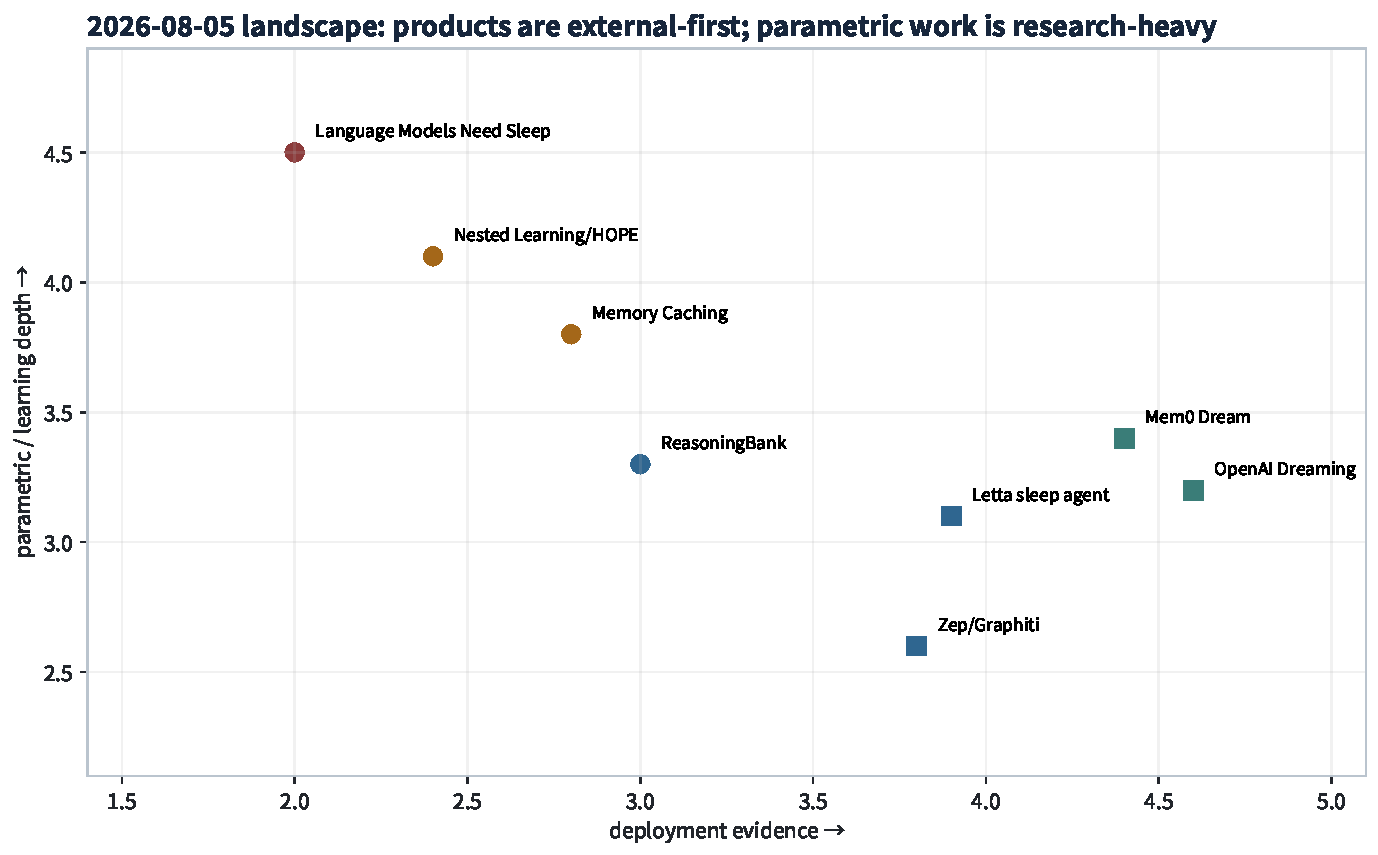
\includegraphics[width=0.96\textwidth]{figures/stc-f014.pdf}
  \caption{Source freeze 시점의 industry--academia landscape. Industry는 external synthesis와
  temporal provenance에, academia는 continual learning, neural memory, learned writer와 capacity
  theory에 더 넓게 분포한다. 좌표는 corpus의 정성적 audit를 시각화한 것이며 시장 규모가 아니다.}
  \stcfigure{STC-F014}
  \figsource{Original synthesis; SRC-STC-0054, SRC-STC-0056, SRC-STC-0057}{제품과 연구 lineages를 external lifecycle, learned memory policy, parametric consolidation, benchmark/theory 축에 배치한 지도.}
  \label{fig:industry-academia}
\end{figure}

Industry에서 가장 분명한 경로는 episode 보존 $\rightarrow$ contradiction/dedup $\rightarrow$
scheduled pattern synthesis $\rightarrow$ future retrieval $\rightarrow$ user control/provenance다.
Academia의 경로는 더 넓다. Replay와 continual-learning regularization, test-time neural memory,
memory writer/router RL, rate--distortion compaction, self-evolving strategy memory, sequential fact
reachability가 서로 다른 이름으로 같은 admission--transform--destination--validation 문제를 만든다.
\autocite{srcstc0020,srcstc0021,srcstc0035,srcstc0043,srcstc0051}

따라서 momentum에 대한 정확한 표현은 ``external background transformation은 I3/E4에 도달했고,
learned external policy는 빠른 E2--E3 frontier이며, broad per-user parametric sleep은 E1--E2''다.
이 세 문장을 하나의 ``STC가 뜬다''로 합치면 투자 방향과 실험 설계가 모두 왜곡된다.

\section{번역 corpus가 담당하는 역할}

전체 source를 모두 번역하는 대신, explicit sleep, biological/computational precursor, continual
learning, external memory, neural memory, capacity, negative evidence를 가로지르는 15편을 balanced
translation corpus로 고정했다.\claim{STC-C004} 번역본은 의견을 추가하는 secondary review가 아니라
원문의 section·figure·limitation을 보존하는 독해 보조물이다. 반면 이 Study는 그 source들을
problem과 lifecycle 기준으로 재조합하는 분석이다. 두 산출물을 분리해야 번역자의 해석이 원저자의
주장처럼 보이지 않는다.

\begin{keypoint}[Evidence trajectory의 결론]
새로운 축의 가장 강한 증거는 하나의 breakthrough paper가 아니다. Continual-learning mechanism,
external-memory product, asynchronous implementation, temporal provenance, realistic benchmark가 서로
다른 층에서 같은 lifecycle boundary를 채우기 시작했다는 점이다. 다만 parametric destination의
장기 retention·delete·rollback·fleet cost를 동시에 보여 주는 공개 증거는 아직 비어 있다.
\end{keypoint}

\chapter{Scaling law: 법칙이 아니라 측정 가능한 가설부터}
\label{STC-S12}

Pre-training scaling은 통제된 data, parameter, compute와 loss의 관계를 다룬다. STC에는 previous
state, wake evidence, admission policy, memory medium, cycle count, future query reuse, validation과
publication이 추가되어 path-dependent하다. 따라서 ``accuracy versus sleep FLOPs'' 한 곡선은 state가
증가했는지, data가 좋아졌는지, future reuse가 달랐는지 구분하지 못한다.

동결 corpus의 어느 source도 보편적인 sleep-time scaling law를 확립하지 않는다.\claim{STC-C041}
\autocite{srcstc0034,srcstc0035,srcstc0050} 아래 식은 \measured{} accounting identity,
\analytical{} break-even, \fitcandidate{}, \hypothesis{}의 네 등급으로 분리한다. 관측 전 가설을
``law''라고 부르지 않는 것이 이 장의 가장 중요한 결과다.

\begin{figure}[htbp]
  \centering
  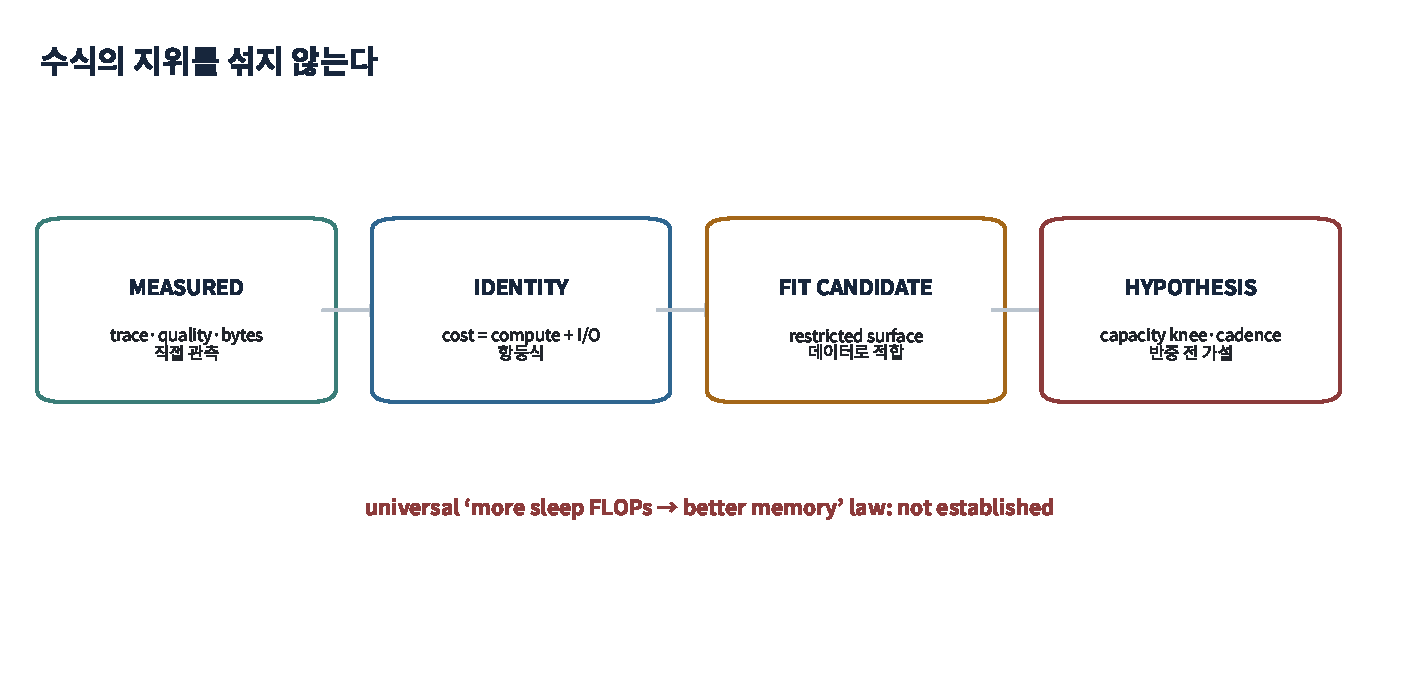
\includegraphics[width=0.98\textwidth]{figures/stc-f007.pdf}
  \caption{Scaling statement의 네 등급. Identity는 장부를 닫고, break-even은 제한된 가정 아래
  경계를 계산하며, fit candidate는 sweep에 맞추고, hypothesis는 반증 실험을 기다린다.}
  \stcfigure{STC-F007}
  \figsource{Original synthesis; SRC-STC-0035, SRC-STC-0050}{측정식에서 보편 법칙으로 갈수록 필요한 가정과 검증 범위가 증가하는 네 단계 사다리.}
  \label{fig:scaling-evidence-ladder}
\end{figure}

\section{State와 lifecycle work를 먼저 닫는 identity}

Answer-bearing retained state를 destination 하나로 축소하면 안 된다.

\begin{equation}
B_{retained}=B_r+B_e+B_l+B_p+B_a+B_v,
\label{eq:retained-state}
\end{equation}

여기서 $B_r$은 canonical/raw evidence, $B_e$는 text/vector/graph/index, $B_l$은 latent·KV·recurrent
state, $B_p$는 adapter/expert/weight delta, $B_a$는 optimizer·importance·router·teacher support,
$B_v$는 lineage·predecessor·rollback state다. Active summary bytes만 보고 ``압축률''을 계산하면 archive와
recovery copy가 사라진 것처럼 보이는 오류가 생긴다.

동시에 존재하는 candidate, pinned predecessor, migration, workspace, replica까지 더한 peak는

\begin{align}
B_{peak,state}(t)={}&B_{retained}(t)+B_{candidate}(t)+B_{pinned}(t)\nonumber\\
&+B_{migration}(t)+B_{workspace}(t)+B_{replica}(t),\\
B_{peak,physical}(t)={}&B_{base,resident}(t)+B_{peak,state}(t)+B_{execution}(t).
\end{align}

Physical maximum은 각 항의 서로 다른 시간대 high-water mark를 더하지 않고 같은 timestamp에서
평가한다. Separate wake/sleep fleet가 contention을 줄이면서 base model replica를 늘릴 수 있으므로
incremental state와 physical placement를 둘 다 보고해야 한다.

Full-history replay는 특히 위험하다. Cycle $t$에서 이전 task의 $m_i$개를 모두 replay하면

\begin{equation}
W_T=\sum_{t=1}^{T}\sum_{i=1}^{t}m_i
=\sum_{i=1}^{T}m_i(T-i+1).
\end{equation}

$m_i=m>0$이면 $W_T=mT(T+1)/2=\Theta(T^2)$다. Admission fraction을 일정 비율 줄이는 것만으로는
계수만 줄고 차수가 바뀌지 않는다. Bounded memory를 주장하려면 expire, compaction, coreset,
generated replay 또는 selective revisit가 실제로 lifetime work와 retained state를 제한하는지 보여야 한다.

\section{Valid reuse가 만드는 compile break-even}

Sleep artifact $i$의 가치에서 raw memory count나 sleep FLOPs보다 유용한 후보 변수는 valid reusable
evidence per lifecycle cost다.\claim{STC-C043}\autocite{srcstc0035,srcstc0043,srcstc0051}
그 이유는 compile이 한 번 비싸도 미래에 반복 사용되면 이득이고, 수천 개 memory를 만들었어도 다시
쓰이지 않으면 이득이 0이기 때문이다.

Stationary하고 quality가 같다는 제한된 가정에서 reuse break-even은

\begin{equation}
n^*=\frac{C_{compile}+C_{maint}}{\Delta C_{use}}.
\label{eq:reuse-break-even}
\end{equation}

Validity survival과 discount를 넣으면 horizon $H$의 expected valid reuse는

\begin{equation}
R_i(H)=\int_0^H \lambda_i(t)S_i(t)e^{-\omega t}\,dt.
\end{equation}

Promotion은 $R_i(H)\Delta U_{ij}$가 compile, serve, governance, risk cost의 합보다 클 때만 후보가 된다.
Future reuse를 oracle로 쓰지 않기 위해 실제 router는 past-only feature로 $\widehat R_i$를 예측하고,
calibration error도 lifecycle cost에 넣는다.

\begin{figure}[htbp]
  \centering
  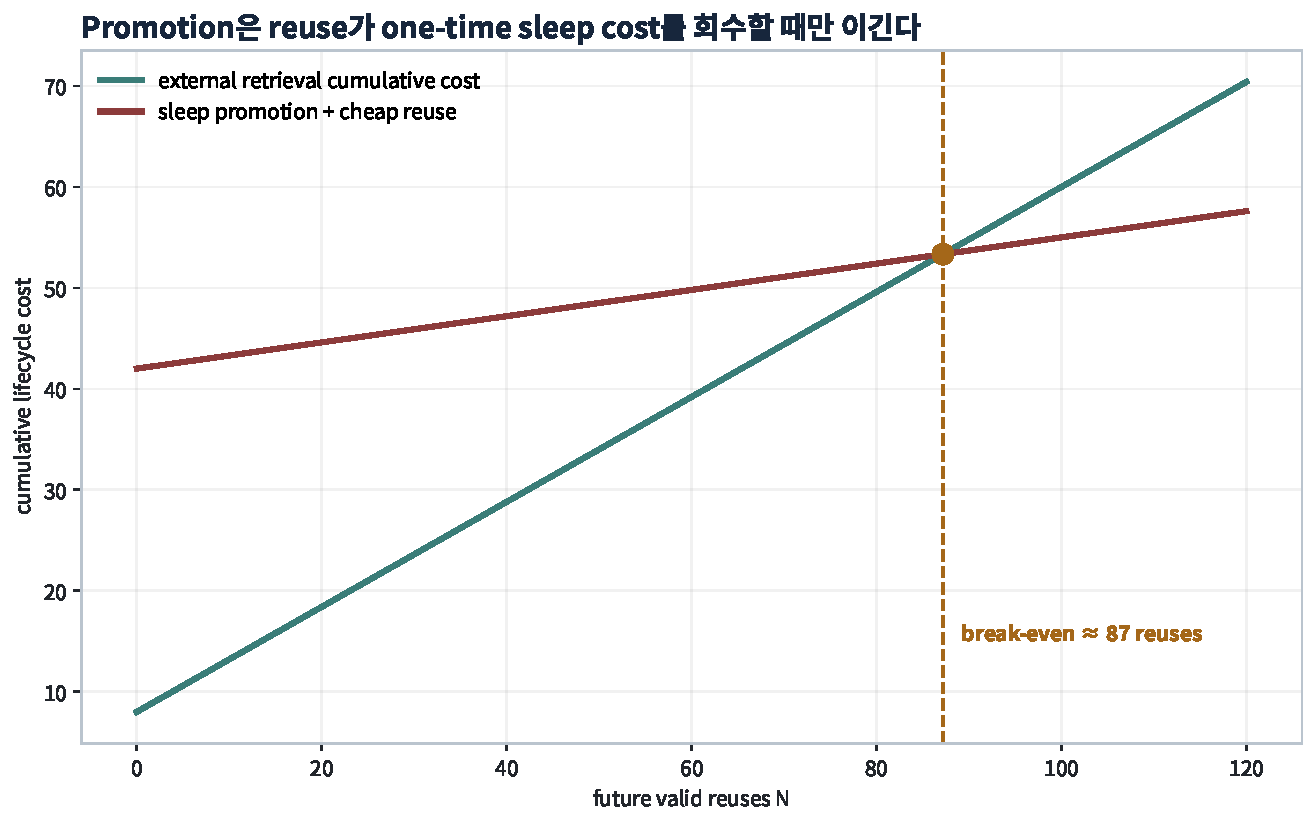
\includegraphics[width=0.96\textwidth]{figures/stc-f008.pdf}
  \caption{One-time sleep cost와 future valid reuse의 analytical crossover. Break-even 왼쪽은 external
  retrieval이, 오른쪽은 compiled artifact가 유리할 수 있다. Quality·governance 차이가 있으면 경계가
  이동한다.}
  \stcfigure{STC-F008}
  \figsource{Original analytical redraw; SRC-STC-0027, SRC-STC-0052}{초기 compile 비용을 수평선으로, reuse에 따라 누적되는 per-use saving을 상승선으로 나타낸 교차 그래프.}
  \label{fig:reuse-break-even}
\end{figure}

측정용 efficiency는 scalar를 강제하지 않고 먼저 Pareto vector로 보고한다.

\begin{align}
\eta_i={}&\frac{\Delta U_{later,i}\,R_{valid,i}}{C_{life,i}},\\
C_{life}={}&C_{ingest}+C_{transform}+C_{train}+C_{validate}\nonumber\\
&+C_{publish}+C_{serve}+C_{maint}+C_{delete/rollback}.
\end{align}

Dollar, joule, byte, second를 임의 환율로 합치지 않는다. Utility floor를 통과한 뒤 비용을 비교하거나,
cost cap 아래 utility를 비교하는 방식이 더 재현 가능하다.

\section{Finite state가 만드는 capacity knee}

고정된 finite state는 positive-entropy stream을 같은 distortion으로 영원히 보존할 수 없다. Mutable state가
$b_{mutable}$ bits이고 conditionally independent answer family의 rate--distortion cost가
$R_{Y_i\mid Q_i,\Theta_0}(D_i)$라면 제한된 조건 아래

\begin{equation}
\sum_{i=1}^{n}R_{Y_i\mid Q_i,\Theta_0}(D_i)
\le H(M_n\mid\Theta_0)\le b_{mutable}.
\end{equation}

이는 facts-per-parameter 보편 상수가 아니다. 하지만 계속 들어오는 novel evidence에 대해 state growth,
distortion 증가, forgetting, external offload 중 적어도 하나가 필요하다는 점은 분명히 한다.

Finite memory에서는 marginal consolidation utility가 떨어지고 interference, compaction 또는 delete cost가
급증하는 capacity knee가 나타날 것으로 예상된다.\claim{STC-C045}
\autocite{srcstc0034,srcstc0035,srcstc0036} Physical storage knee, normal-query reachability knee,
retrieval index knee, new-task plasticity knee, governance knee, hot-state residency knee는 서로 다른 위치에
있을 수 있다. 따라서 ``parameter가 아직 남았다''는 말은 behavioral capacity의 반증이 아니다.

\begin{figure}[htbp]
  \centering
  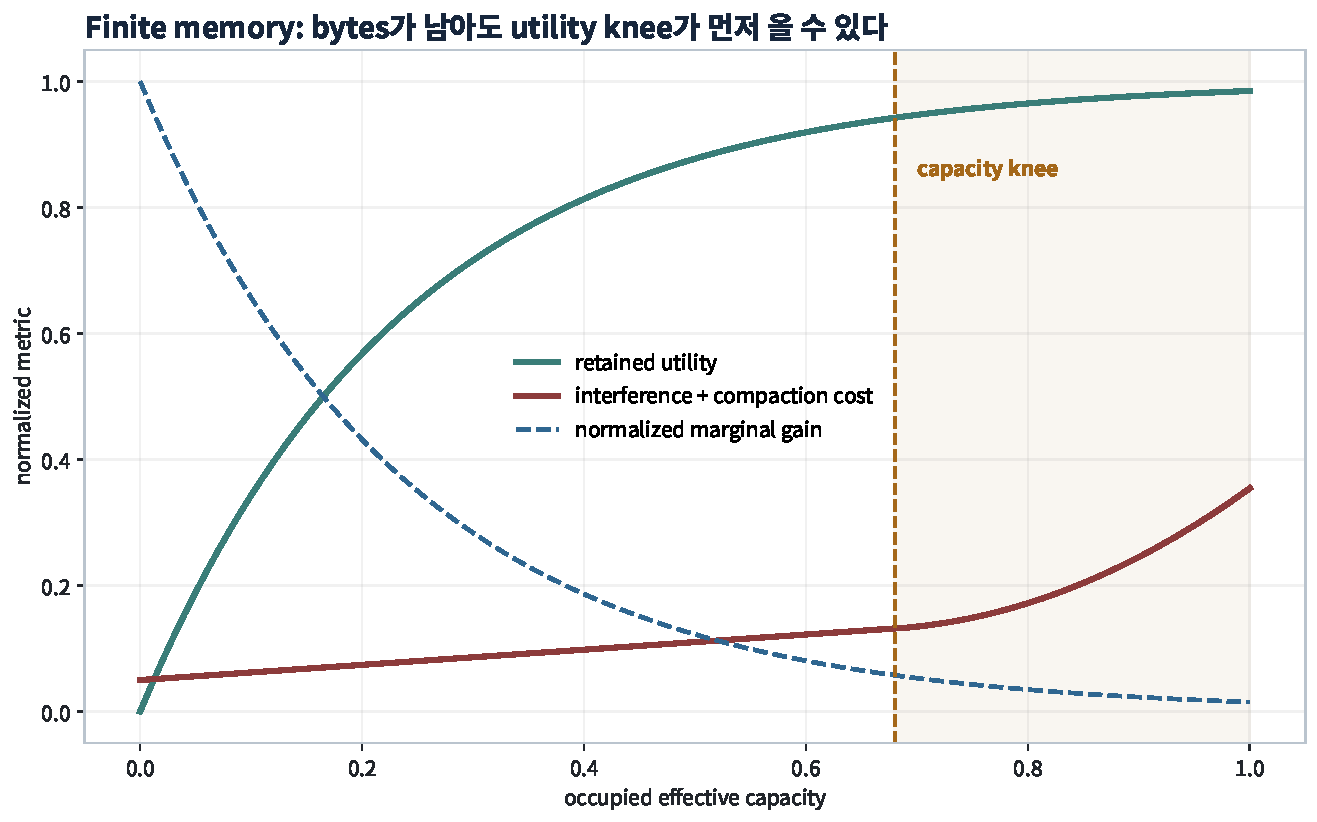
\includegraphics[width=0.96\textwidth]{figures/stc-f009.pdf}
  \caption{Finite-memory capacity knee의 가설적 형태. Physical occupancy가 한계에 닿기 전에 behavioral
  reachability 또는 plasticity가 임계값 아래로 내려갈 수 있다. 곡선은 설명용이며 측정 결과가 아니다.}
  \stcfigure{STC-F009}
  \figsource{Original hypothesis redraw; SRC-STC-0034, SRC-STC-0036}{Evidence load가 증가할 때 retention과 plasticity가 서로 다른 knee에서 감소하는 두 곡선.}
  \label{fig:capacity-knee}
\end{figure}

Controlled sweep에서는 retention threshold $\tau_{ret}$을 먼저 고정하고

\begin{equation}
\operatorname{logit}p_{ret}(N_a)=\operatorname{logit}\tau_{ret}
-\kappa\log(N_a/K_{eff})
\end{equation}

같은 segmented knee candidate와 generalized mean, min-bottleneck, monotone nonparametric competitor를
함께 맞춘다. 전 구간 power law 하나를 강제하지 않는다.

\section{Cadence와 queue의 내부 optimum}

Optimal cadence는 staleness, batching efficiency, interference와 wake-SLA impact를 균형시켜야 한다.
Continuous update나 무한히 긴 batch 어느 쪽도 일반적으로 최적이 아니다.\claim{STC-C044}
\autocite{srcstc0020,srcstc0022,srcstc0063}

Run cost $C_s$, interval $\tau$, smooth staleness penalty $a\tau^p$라는 제한에서

\begin{equation}
\bar C(\tau)=\frac{C_s}{\tau}+a\tau^p,
\qquad
\tau^*=\left(\frac{C_s}{ap}\right)^{1/(p+1)}.
\label{eq:cadence-optimum}
\end{equation}

Event rate $r_e$, fixed job cost $F$, linear delay harm $h$이면
$\tau^*=\sqrt{2F/(hr_e)}$다. Burst arrival, hard deadline, multi-resource blocking, capacity-triggered
regime change에서는 이 closed form이 깨진다. 이때 queue recursion
$Q_{t+1}=\max\{0,Q_t+A_t-S_t\}$와 P99 job age를 직접 시뮬레이션해야 한다.

\begin{figure}[htbp]
  \centering
  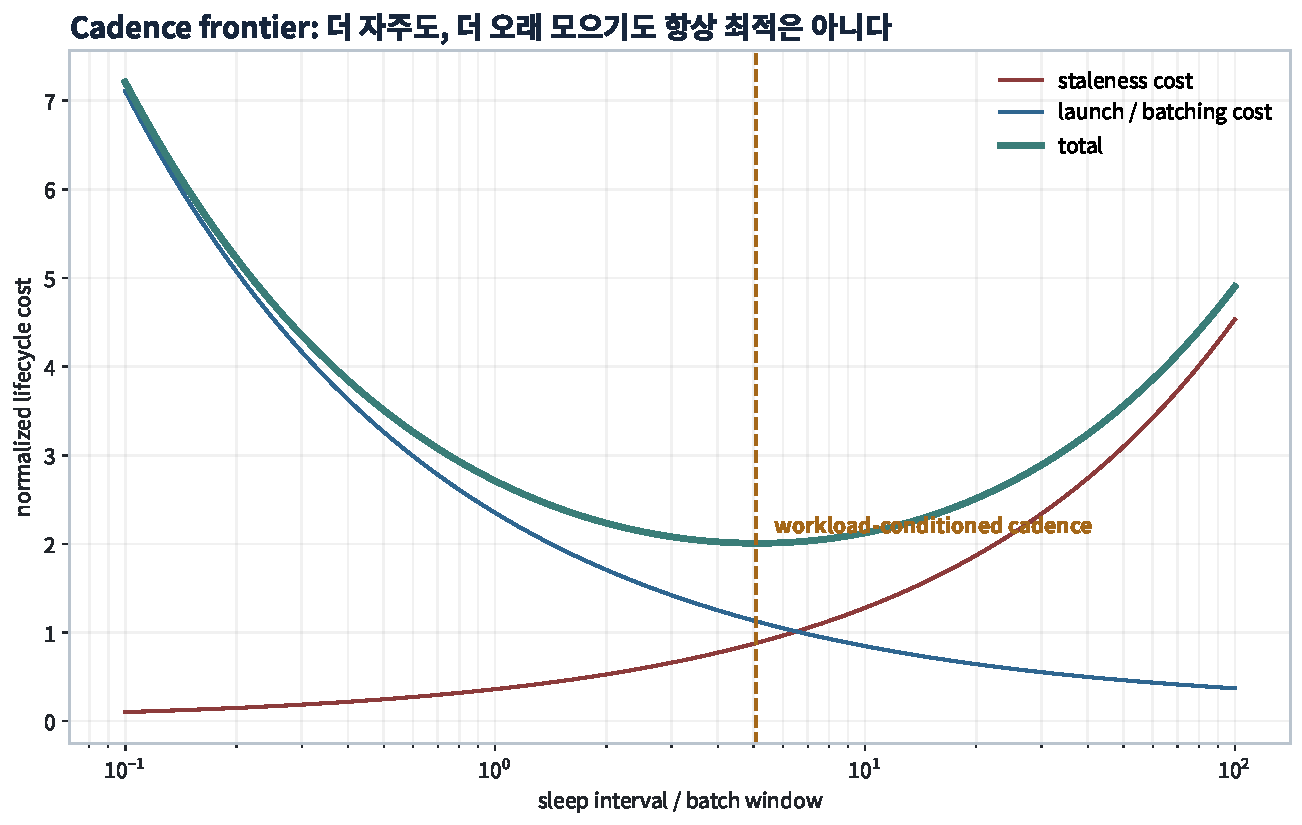
\includegraphics[width=0.96\textwidth]{figures/stc-f010.pdf}
  \caption{Cadence frontier. 너무 잦은 sleep은 fixed overhead와 interference가 크고, 너무 늦은 sleep은
  staleness와 queue age가 크다. 내부 optimum의 위치는 workload와 resource vector에 따라 변한다.}
  \stcfigure{STC-F010}
  \figsource{Original analytical redraw; SRC-STC-0020, SRC-STC-0063}{짧은 interval의 batching 비용과 긴 interval의 staleness 비용이 합쳐져 U자 total cost를 만드는 그래프.}
  \label{fig:cadence-frontier}
\end{figure}

\section{Fit candidate와 법칙 승격 조건}

첫 fit candidate는 saturating return에 interference, staleness, risk penalty를 분리한다.

\begin{equation}
\Delta U=A\left[1-\exp\left(-kF_s^{\alpha}E_{eff}^{\beta}R_v^{\gamma}\right)\right]
-\Phi_{int}-\Phi_{stale}-\Phi_{risk}.
\end{equation}

$E_{eff}$는 authorization, confidence, diversity를 통과한 canonical evidence이고 $R_v$는 valid future
reuse다. Competitor는 log-linear, floor가 있는 power law, segmented knee, generalized mean,
nonparametric monotone surface다. Sign change나 knee가 보이면 global power law를 기각한다.

진짜 STC scaling law라 부르려면 (1) unit과 state boundary를 고정하고, (2) model size·workload·medium·
hardware를 둘 이상 포함하며, (3) strongest alternative와 total lifecycle cost를 맞추고, (4) held-out
condition을 예측하고, (5) knee를 숨기지 않으며, (6) contamination·recursive depth·capacity·cycle control을
통과하고, (7) 실패한 형태를 공개해야 한다. 그 전까지의 정직한 산출물은 identity, restricted
break-even, workload-conditioned empirical surface와 falsifiable hypothesis다.

\chapter{System infrastructure: wake, sleep, memory를 어떻게 잇는가}
\label{STC-S13}

세 개의 logical plane이 곧 세 개의 physical cluster를 뜻하지 않는다. 필요한 것은 latency-critical wake
execution, throughput-oriented candidate construction, transactional publication의 책임 분리다. Load와
state locality가 허용하면 같은 accelerator pool을 time-partition할 수 있고, contention 또는 privacy가
크면 분리할 수 있다. 배치는 brain analogy가 아니라 bytes, queue, SLO 측정으로 결정한다.

\section{세 plane과 하나의 publication transaction}

\begin{enumerate}
  \item \textbf{Wake plane}: inference, retrieval, optional fast learning, event append를 latency SLO 안에서
  수행하고, 하나의 authorized serving head를 pin한다.
  \item \textbf{Sleep plane}: immutable wake snapshot을 읽어 extract, compact, graph update, replay,
  distill, adapter tune, policy update, rebuild, verify job을 수행한다. 결과는 candidate일 뿐 live state가
  아니다.
  \item \textbf{Memory/control plane}: raw evidence와 derived views의 lineage, version, authorization,
  capacity, atomic publish, rollback을 관리한다.
\end{enumerate}

Sleep transaction은 다음처럼 표현할 수 있다.

\begin{equation}
T(X_v,M_v,B,P)\rightarrow \widehat M_{v+1}
\xrightarrow[\text{compare-and-swap}]{\text{validate}} M_{v+1}.
\label{eq:sleep-transaction}
\end{equation}

$X_v$는 immutable event range, $M_v$는 published manifest, $B$는 resource budget, $P$는 frozen policy다.
Candidate는 old/new/safety/delete/poison/system canary를 통과한 뒤에만 manifest-last로 publish된다.
Reader는 요청 중 한 version을 보며 partial vector/metadata/adapter state를 섞어 보지 않는다.

\section{Source-of-record와 heterogeneous materialized views}

Derived memory의 governance basis로는 updated weights 하나보다 external source-of-record와 provenance
graph가 강하다.\claim{STC-C046}\autocite{srcstc0053,srcstc0063,srcstc0066} Raw event도 retention
policy가 허용하는 동안만 canonical이다. Text summary, vector, graph, latent/KV, adapter, shared weight는
모두 source lineage를 가진 materialized view로 취급한다.

\begin{table}[htbp]
\centering
\caption{Memory medium별 serving path와 rollback contract}
\label{tab:medium-contract}
\begin{tabularx}{\textwidth}{L{0.18\textwidth} L{0.20\textwidth} Y L{0.24\textwidth}}
\toprule
Medium & Wake path & Update/validation & Rollback basis \\
\midrule
raw episode & selective retrieval & append, redact, expire & event/version log \\
semantic text & prompt injection & rewrite, faithfulness & source span + predecessor \\
vector/graph & ANN/traversal & re-embed, edge validity & index generation + episode \\
latent/recurrent & accelerator state read & compatibility, semantic probe & checkpoint or source rebuild \\
adapter/expert & model forward/router & train, merge, old/new canary & base digest + delta version \\
shared weight & model forward & full regression/unlearning & checkpoint + training lineage \\
\bottomrule
\end{tabularx}
\end{table}

삭제는 tombstone 한 번이 아니다. Immediate access deny, online artifact invalidation, derived lineage rebuild,
backup/key expiry, behavioral residual test를 서로 다른 deadline으로 기록한다. Old checkpoint 전체를 되살리는
rollback은 그 사이의 delete/consent epoch를 되돌릴 수 있으므로, authorized sub-root만 새 generation으로
재조합해야 한다.

\section{Scheduler: operator, destination, cadence를 분리한다}

하나의 evidence region에 대한 action space는 NO\_OP, RETAIN\_EXACT, EXPIRE, DEDUP, MERGE,
ABSTRACT, GRAPH\_UPDATE, LATENT\_COMPILE, ADAPTER\_COMPILE, PARAMETRIC\_PROMOTE, DEMOTE,
REBUILD, QUARANTINE를 포함한다. Learned policy가 action을 제안해도 privacy, tenant boundary,
capacity, deadline, promotion gate는 hard constraint로 남긴다.

Batching key는 base model/tokenizer와 adapter shape, embedding/index version, privacy zone, deadline,
operator, source shard다. 같은 batch가 효율적이라는 이유로 tenant security domain을 합치지 않는다.
Preemption은 uncommitted candidate를 버릴 수 있어야 하고, wake saturation 시 sleep보다 wake가 우선한다.

Sleep service는 scalar FLOP queue가 아니라 resource vector queue다.

\begin{equation}
\mathbf c_j=(c_{GPU\text{-}s},c_{CPU\text{-}s},c_{HBM\text{-}byte\text{-}s},
c_{RAM\text{-}byte\text{-}s},c_{IO\text{-}byte},c_{net\text{-}byte}).
\end{equation}

Mean GPU utilization이 낮아도 source affinity, validation model, index lock, network link 때문에 P99 job age가
발산할 수 있다. Queue 안정성은 utilization 한 숫자뿐 아니라 privacy deadline과 tenant starvation으로
판정한다.

\section{State migration roofline}

Separate sleep cluster는 training accelerator utilization을 높일 수 있지만 source episode, base model,
optimizer, adapter candidate, validation trace를 이동시킨다. Link $\ell$마다 이동 bytes $B_\ell$, transfer
price/energy $p_\ell$, delay $T_\ell$, delay value $v_{delay}$를 두면

\begin{equation}
C_{move}=\sum_{\ell}\left(B_\ell p_\ell+T_\ell v_{delay}\right).
\end{equation}

추가 local execution과 replication cost가 $C_{move}$보다 작을 때만 compute를 data 쪽으로 옮긴다.
Model/optimizer residency가 source보다 훨씬 크면 centralized GPU가, source-to-delta ratio와 privacy locality가
크면 shard-local preprocessing이 유리할 수 있다.

\begin{figure}[htbp]
  \centering
  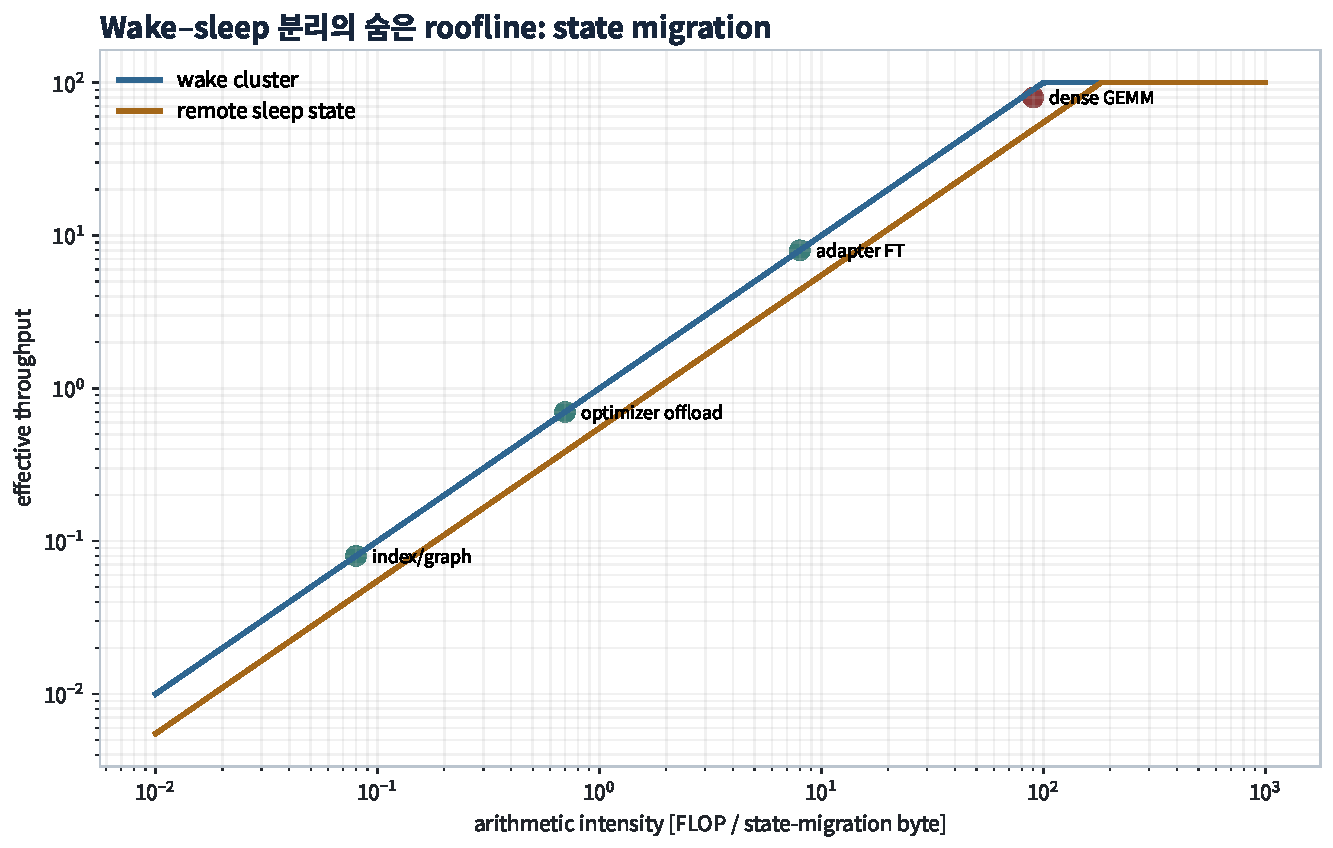
\includegraphics[width=0.97\textwidth]{figures/stc-f011.pdf}
  \caption{Wake/sleep placement의 state-migration roofline. Arithmetic intensity가 아니라 유용한 sleep
  work 대비 이동 state의 비율과 link bandwidth가 placement crossover를 정한다. 표시된 영역은 설계
  공간이며 특정 GPU의 측정 결과가 아니다.}
  \stcfigure{STC-F011}
  \figsource{Original systems synthesis; SRC-STC-0022, SRC-STC-0059}{Shared, separate, shard-local 배치를 state movement와 compute efficiency 축에서 비교한 roofline형 지도.}
  \label{fig:state-migration-roofline}
\end{figure}

\section{네 가지 physical placement}

\begin{longtable}{L{0.18\textwidth} L{0.22\textwidth} L{0.24\textwidth} L{0.21\textwidth}}
\caption{Physical placement option과 측정해야 할 trade-off}\label{tab:placement-options}\\
\toprule
Placement & 장점 & 비용/위험 & 적합 조건 \\
\midrule
\endfirsthead
\toprule
Placement & 장점 & 비용/위험 & 적합 조건 \\
\midrule
\endhead
shared priority fleet & base/model copy 최소, pooling & wake tail contention & sleep가 작고 preemptible \\
time-partitioned fleet & idle window 활용 & burst와 timezone mismatch & predictable diurnal load \\
separate wake/sleep & isolation, training batch 효율 & base replica와 network movement & sustained sleep demand \\
regional/shard-local hybrid & source locality, privacy & 낮은 local compute efficiency, fragmentation & source-to-delta ratio가 큼 \\
\bottomrule
\end{longtable}

\section{운영 계약}

Minimum viable system은 (1) append-only event log, (2) exact snapshot, (3) copy-on-write candidate,
(4) signed validation result, (5) atomic serving-head swap, (6) delete epoch와 deny root, (7) version-pinned
read, (8) bounded rollback과 GC owner를 가져야 한다. Algorithm quality가 좋아도 이 계약이 없으면 wake
request가 half-published state를 읽고, deleted source가 predecessor에서 부활하며, sleep retry가 duplicate
update를 만들 수 있다.

\begin{keypoint}[Infra 결론]
필요한 분리는 cluster의 개수가 아니라 responsibility와 transaction boundary다. Wake는 응답과 event
capture, sleep은 candidate construction, memory/control은 authoritative lineage와 publication을 담당한다.
Data 이동을 최소화한다는 말은 source만 보는 것이 아니라 base, optimizer, candidate, validation,
predecessor까지 같은 timestamp와 link에서 계측한다는 뜻이다.
\end{keypoint}

\chapter{Falsifiable benchmark와 experiment roadmap}
\label{STC-S15}

이 분야에 필요한 다음 산출물은 더 큰 metaphor가 아니라 matched lifecycle experiment다. 같은 wake
events와 future queries를 주고, exact external retention, external compaction, latent/KV compilation,
user-local adapter, deliberate forgetting, past-only hybrid routing 중 무엇이 가장 나은지를 측정해야 한다.
Null result와 boundary를 계획에 포함해야 negative paper도 가치가 있다.

\begin{figure}[htbp]
  \centering
  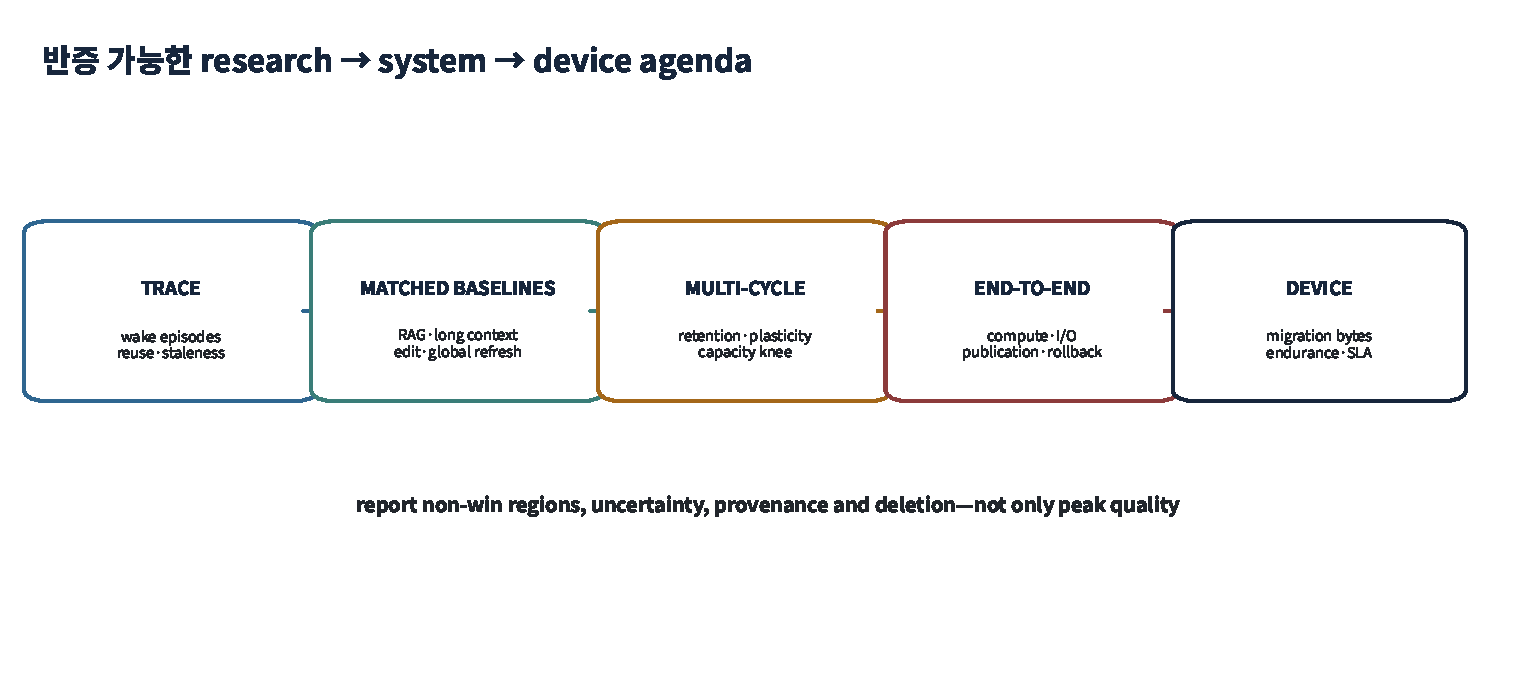
\includegraphics[width=0.98\textwidth]{figures/stc-f015.pdf}
  \caption{Falsifiable research agenda. Evidence stream, candidate construction, lifecycle validation,
  repeated-cycle evaluation, scaling fit을 하나의 provenance chain으로 연결한다.}
  \stcfigure{STC-F015}
  \figsource{Original synthesis; SRC-STC-0036, SRC-STC-0050, SRC-STC-0056}{Matched methods, cycle probes, systems/governance metrics, held-out scaling test가 순차적으로 이어지는 roadmap.}
  \label{fig:benchmark-agenda}
\end{figure}

\section{독립 단위와 cycle}

최상위 independent unit은 user/stream이다. Cycle과 probe를 독립 sample처럼 세어 significance를
부풀리지 않는다. 한 cycle은 다음 순서를 가진다.

\begin{align*}
\text{wake capture}&\rightarrow\text{pre-sleep probe}\rightarrow
\text{immutable snapshot}\rightarrow\text{candidate}\\
&\rightarrow\text{validate/publish}\rightarrow\text{post-sleep probe}
\rightarrow\text{delayed next-wake probe}.
\end{align*}

Default horizon은 128 cycles, sensitivity는 $C\in\{8,32,128,512\}$, retrieval lag는 가능한 경우
$\{1,8,32,128\}$ cycles로 둔다. 단일 sleep 후 정확도는 lifelong behavior를 지지하지 못한다.

\section{Observable과 oracle을 물리적으로 분리한다}

Method가 보는 observable stream에는 event payload, 현재 confidence, privacy scope, 알려진
supersession/delete, past reuse, resource/queue state만 있다. True future reuse, future contradiction,
future deletion, poison truth, ground-truth dependency, clairvoyant destination은 oracle ledger에 따로 둔다.
파일, schema, API permission과 process boundary로 누출을 막는다.

Train은 learned router/compiler를 fit하고, CALIBRATION은 threshold, cadence, baseline hyperparameter를
한 번 선택하며, TEST는 G2 freeze 뒤 한 번만 실행한다. TEST family identity나 future reuse로 configuration을
바꾸는 mutation test가 통과해야 한다. Dream-generated probe도 evaluation query가 아니라 derived training
artifact이므로 generator/prompt/input/output/filter digest를 남긴다.

\section{Event와 query family}

\begin{table}[htbp]
\centering
\caption{독립적으로 변화시킬 event factor와 주요 failure}
\label{tab:event-families}
\begin{tabularx}{\textwidth}{L{0.23\textwidth} L{0.34\textwidth} Y}
\toprule
Family & Controlled variables & 잡아야 할 failure \\
\midrule
stable exact fact & entropy, surface length, reuse, lag & semantic compression이 exact detail을 지움 \\
volatile fact/preference & validity interval, correction hazard & stale overwrite, historical loss \\
procedure/skill & reusable/one-off, environment version & vague summary, non-executable memory \\
relation/graph & alias, temporal edge, hop count & entity collision, invalid edge \\
failure feedback & wrong action, correction, avoidance & success-only bias \\
privacy/delete & consent expiry, dependency fan-out & tombstone-only delete \\
poison/adversarial & injection, conflicting frequency, delayed label & poison amplification \\
one-off distractor & salience, payload size, zero reuse & unnecessary consolidation \\
\bottomrule
\end{tabularx}
\end{table}

Reuse, volatility, poison, deletion, payload size와 memory pressure는 서로 독립적으로 변화시킨다. Query는
exact, semantic, temporal, relational, procedural, negative/failure, calibration, deletion family로 나눈다.
Acquisition query, exact repeat, held-out paraphrase, held-out composition, correction probe, unrelated control을
동일 지표로 합치지 않는다. ``기억한 문장을 그대로 다시 답했다''와 ``새 상황에 procedure를 적용했다''는
다른 능력이다.

\section{Confirmatory methods와 resource envelope}

Primary deployable family는 raw external, compressed external, latent/KV compiler, user-parametric LoRA,
static mixture, past-only hybrid router 여섯 개다. Clairvoyant oracle은 heterogeneity의 upper bound일 뿐
deployable method가 아니다. Long-context no-memory lower bound와 unbounded full-history upper bound는
diagnostic으로 남긴다.

모든 method는 다음 upper bound를 공유한다.

\begin{itemize}
  \item live token, active byte, durable byte, total incremental peak-state byte,
  \item physical HBM/fleet peak, sleep FLOPs, peak accelerator,
  \item 동일한 information cutoff, privacy와 delete contract.
\end{itemize}

Search/tuning, router, judge, embedding, synthetic data, optimizer, answer-reachable KV/recurrent state, index
rebuild, raw archive, lineage, rollback reserve와 transient workspace를 모두 charge한다. 사용하지 않은 budget은
낭비하도록 강제하지 않고 그대로 보고한다.

Reuse $R\in\{0,1,4,16\}$와 active-capacity ratio
$\phi\in\{1,1/4,1/16\}$을 교차한다. Schedule/operator factorial은 inline versus deferred와 identity
versus semantic consolidation을 destination external로 고정해, execution timing의 효과와 추가 정보를 더
본 효과를 분리한다.

\section{Metric stack}

\begin{longtable}{L{0.17\textwidth} L{0.74\textwidth}}
\caption{한 결과표에 함께 있어야 할 metric stack}\label{tab:benchmark-metrics}\\
\toprule
Layer & Required metrics \\
\midrule
\endfirsthead
\toprule
Layer & Required metrics \\
\midrule
\endhead
learning & lifetime utility AUC, current utility, acquisition, retention/forgetting, forward transfer, memory half-life \\
semantic & exact/semantic/temporal/relational/procedural, composition, relevance, calibration, false memory \\
memory path & writer/retriever/reader error, route/merge compatibility, coverage, faithfulness, detail loss, stale conflict \\
robustness & poison amplification, cross-user/task interference, rare-tail survival, recursive-depth distortion \\
governance & access deny, physical removal, lineage invalidation, key expiry, behavioral residual, rollback success/time \\
serving & TTFT/ITL/task P50/P95/P99, throughput, cache/adapter hit, load/swap, fallback \\
sleep service & throughput, queue age, deadline miss, retry, validation/publish/rollback cost \\
resources & pre/post/wake/sleep/validation FLOPs, retained/peak bytes, bytes moved by link, write amplification, energy \\
compatibility & base/tokenizer/embedding version, artifact route, rebase and rebuild cost \\
\bottomrule
\end{longtable}

Primary quality endpoint은 cycle과 pre/post/delayed probe block에 동일 가중치를 주는 lifetime utility AUC다.
Energy-per-correct는 frozen accuracy floor 위에서만 계산한다. Delete score는 access denial과 physical removal,
derived invalidation, behavioral residual을 한 binary로 합치지 않는다.

\section{통계·재현성과 claim-down rule}

모든 method는 같은 stream, event order, query order, resource tuple을 받는다. User/stream을 paired resampling
unit로 사용하고 workload-family$\times$seed-family block을 유지한다. Hardware placement와 method order는
randomize 또는 block한다. Outcome을 본 뒤 stopping point, comparator, hypothesis family를 바꾸지 않는다.

Run artifact는 source/version $\rightarrow$ question/hypothesis $\rightarrow$ config/data/code/environment
$\rightarrow$ raw checksum $\rightarrow$ result $\rightarrow$ claim $\rightarrow$ figure/table
$\rightarrow$ manuscript sentence를 연결한다. Timeout, OOM, deadline miss, cap violation은 missing data가
아니라 consumed work를 charge한 RESOURCE\_FAILURE로 처리한다.

다음 경우 claim을 낮춘다: effect가 materiality margin보다 작음, equivalence interval이 margin을 걸침,
simulation으로 absolute hardware latency를 말함, archive를 남기고 total compression이라 함, behavioral
forgetting을 physical deletion이라 함, post-hoc arm을 추가함. Minimum publishable result는 hybrid가
실패해도 deterministic leakage-tested stream, matched methods, complete resource ledger, retention/acquisition
분리와 잘 추정된 crossover·knee·null 중 하나를 남기는 것이다.

\begin{keypoint}[실험의 최종 질문]
``Sleep이 정확도를 높였는가?''가 아니라 ``동일한 evidence와 lifetime budget에서, 어떤 admission,
operator, destination, cadence가 later-wake utility와 governance의 Pareto frontier를 움직였는가?''를 묻는다.
\end{keypoint}

\chapter{Limitations, negative evidence와 falsifiers}
\label{STC-S16}

이 Study의 결론은 2026-08-05 공개 evidence에 대한 조건부 synthesis다. Product 내부 trace, 비공개
deployment incident, 실제 device workload가 없으며, 논문 간 model·task·budget이 달라 meta-analysis를
수행하지 않았다. Original figure의 좌표와 scenario는 측정 결과가 아니라 reasoning aid다.

\section{문헌 자체의 한계}

명시적 parametric sleep 연구는 direct mechanism evidence지만 model scale, task diversity, cycle count와
production governance가 제한된다. Product documentation은 background phase의 존재를 보여도 strongest
alternative 대비 causal advantage를 보여 주지 않는다. Continual-learning precursor는 forgetting을 줄이는
방법을 제공하지만 LLM agent의 deletion, state migration, future reuse economics를 직접 측정하지 않는다.

DANN/SSRN record는 동결 source에서 independent verification에 필요한 method와 result를 충분히 공개하지
않아 load-bearing evidence로 사용하지 않았다.\claim{STC-C047}\autocite{srcstc0039} 제목이나 abstract가
``zero forgetting''을 말해도 full method, data, comparator, statistics, artifact가 없으면 central claim을
지탱할 수 없다. 이 판단은 논문이 틀렸다는 결론이 아니라 증거 접근성에 대한 claim-down이다.

\section{Negative evidence가 가리키는 구조적 위험}

\begin{longtable}{L{0.20\textwidth} L{0.31\textwidth} L{0.39\textwidth}}
\caption{실패 mode와 필요한 control}\label{tab:negative-evidence}\\
\toprule
Risk & 관찰/이론적 근거 & 필요한 control \\
\midrule
\endfirsthead
\toprule
Risk & 관찰/이론적 근거 & 필요한 control \\
\midrule
\endhead
behavioral unreachability & sequential fact가 weights에 남아도 normal query에서 접근 불가 & direct, prompted, compositional reachability를 분리 \\
catastrophic interference & new update가 old task와 plasticity를 손상 & old/new/safety slice, replay/regularization/isolation ablation \\
recursive-data collapse & synthetic-only generations가 rare tail을 잃을 수 있음 & canonical anchor, recursive depth, common/tail distortion \\
false merge/compaction & summary가 exact, temporal, negative detail을 지움 & source spans, faithfulness, exact/temporal query, rebuild \\
memory poisoning & persistent record가 후속 behavior를 조종 & provenance, quarantine, poison canary, least privilege \\
delete illusion & tombstone 뒤 summary, index, cache, adapter에 영향 잔존 & lineage fan-out, deny root, physical removal, residual probe \\
state fan-out & user/cohort artifact와 catalog가 base saving을 상쇄 & total state, hot residency, route/load latency \\
queue/SLA failure & 평균 utilization 전에도 affinity·validation이 P99 age를 악화 & multi-resource queue, deadline, wake preemption \\
version churn & base/tokenizer/embedding 변경이 artifact를 무효화 & compatibility digest, rebase/rebuild cost \\
\bottomrule
\end{longtable}

\begin{figure}[htbp]
  \centering
  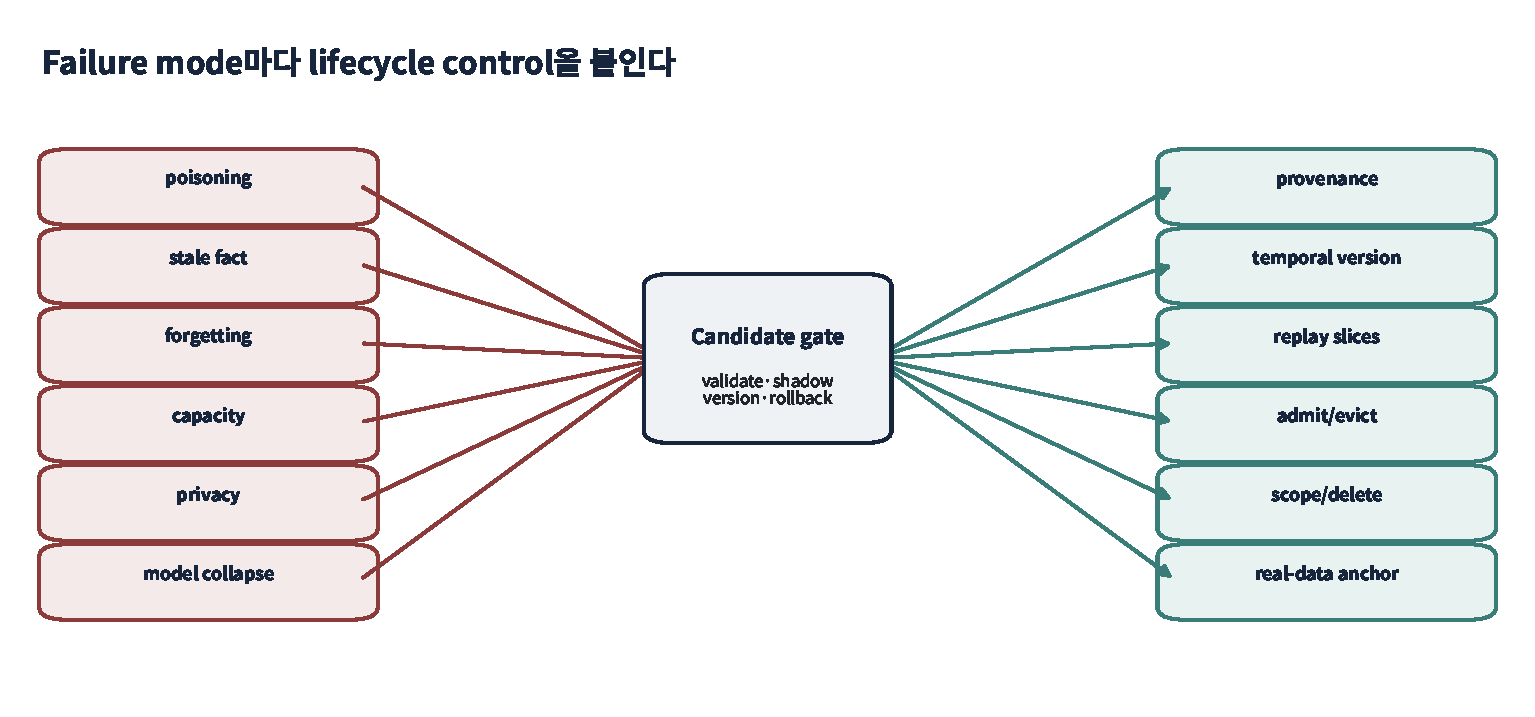
\includegraphics[width=0.98\textwidth]{figures/stc-f013.pdf}
  \caption{Wake capture에서 deletion까지 이어지는 주요 failure mode와 lifecycle control. 한 단계의
  accuracy gate만으로는 poison, stale publish, rollback resurrection, residual delete를 막을 수 없다.}
  \stcfigure{STC-F013}
  \figsource{Original synthesis; SRC-STC-0042, SRC-STC-0053}{Admission, candidate, publish, serve, delete 단계마다 poison·interference·race·residual과 대응 control을 연결한 흐름도.}
  \label{fig:failure-controls}
\end{figure}

\section{결론을 뒤집거나 좁힐 구체적 falsifier}

\textbf{F1---새 phase claim.} 동일 transformation, information cutoff, destination, total resource를
맞췄을 때 deferred와 synchronous 실행의 later-wake quality, wake-SLA, batching 차이가 모두 사라지면
``새 scientific axis''는 scheduling label로 좁혀야 한다.

\textbf{F2---hybrid recommendation.} External-only 또는 direct parametric-only가 stable skill과 volatile
fact 모두에서 utility, cost, deletion, rollback, portability를 지배하면 hybrid default를 폐기한다.

\textbf{F3---valid-reuse hypothesis.} Reuse와 query predictability를 넓게 sweep해도 STC gain과 interaction이
없거나 predictor error가 top-$k$ yield를 없애면 reuse-based promotion 이론을 기각한다.

\textbf{F4---capacity knee.} Repeated stream에서 behavioral retention/plasticity가 physical occupancy와
같이 부드럽게 변하고 앞선 knee가 재현되지 않으면 별도 behavioral knee hypothesis를 기각한다.

\textbf{F5---canonical anchoring.} Synthetic/summary replay와 source-anchored replay의 rare-tail survival이
matched cost에서 차이가 없으면 canonical anchor의 안정성 주장을 낮춘다.

\textbf{F6---dedicated sleep infra.} Shared priority fleet가 모든 realistic trace에서 더 낮은 physical
peak, 이동 bytes, P99 wake latency와 job age를 동시에 보이면 separate sleep cluster 필요성을 기각한다.

\textbf{F7---device relevance.} Background memory job이 commodity CPU/object-store metadata 수준에 머물고
retained bytes, rewrite, movement, tail-SLA가 장치 선택에 영향을 주지 않으면 새로운 memory workload라는
주장을 좁힌다.

\section{Coverage와 saturation의 한계}

Search cluster는 date-bounded snapshot이며 five active frontier와 five measurement gap을 명시적으로
남겼다. 특히 Google, Meta, Microsoft의 research output은 넓지만 public production per-user weight sleep의
부재를 ``그 회사가 하지 않는다''는 negative fact로 바꾸지 않는다. 공개하지 않았을 가능성과 아직
측정하지 않은 possibility가 있기 때문이다.

Figure는 권리 검토된 original redraw만 사용했으며 source paper figure를 직접 복제하지 않았다. 이
선택은 copyright risk를 줄이지만 원 실험 plot의 numeric fidelity를 대신하지 않는다. 독자는 claim
ledger와 primary source로 수치를 확인해야 한다.

\section{본 논문이 주장하지 않는 것}

\begin{itemize}
  \item Biological NREM/REM stage가 AI operator에 one-to-one으로 대응한다는 주장,
  \item 더 많은 sleep FLOPs가 항상 utility를 높인다는 universal monotone law,
  \item weights가 external memory보다 본질적으로 더 장기적이라는 주장,
  \item 공개 product lifecycle가 comparative scientific optimality를 입증한다는 주장,
  \item simulation이 특정 GPU·memory device의 latency, energy, endurance를 측정했다는 주장,
  \item P3-held device hypothesis가 publication 또는 patent review를 통과했다는 주장.
\end{itemize}

\begin{cautionbox}[가장 중요한 한계]
현재 논문은 measurement program과 conditional strategy를 제시한다. STC의 universal dominance나 broad
parametric deployment를 관측한 논문이 아니다. 이 구분을 유지해야 향후 negative result가 연구 실패가
아니라 이론의 경계를 좁히는 결과가 된다.
\end{cautionbox}


\appendix
% Generated from claims/stc-study/claim-map.json. Do not edit by hand.
\chapter*{Canonical claim–evidence ledger}
\addcontentsline{toc}{chapter}{Canonical claim–evidence ledger}
\markboth{Canonical claim–evidence ledger}{Canonical claim–evidence ledger}
본문의 파란 claim ID는 이 표의 canonical English statement와 source locator로 연결된다.
이 표는 번역문이 아니라 Veridraft gate를 통과한 frozen assertion surface다.

\scriptsize
\begingroup
\setlength{\tabcolsep}{3pt}
\begin{longtable}{p{0.105\textwidth} p{0.105\textwidth} p{0.455\textwidth} p{0.245\textwidth}}
\caption{Veridraft-gated public claims (source freeze 2026-08-05)}\label{tab:claim-ledger}\\
\toprule
ID & Type / confidence & Canonical claim & Evidence locator \\
\midrule
\endfirsthead
\toprule
ID & Type / confidence & Canonical claim & Evidence locator \\
\midrule
\endhead
\midrule\multicolumn{4}{r}{다음 쪽에 계속}\\
\endfoot
\bottomrule
\endlastfoot
\hypertarget{claim-ledger:STC-C001}{\hyperlink{claim:STC-C001}{\textbf{STC-C001}}} & direct fact\newline high & The date-frozen evidence audit contains 73 primary papers, official releases, documentation pages, and tagged repositories. & \texttt{SRC-STC-0014}: source registry audit; entry SRC-STC-0014 \\
\hypertarget{claim-ledger:STC-C002}{\hyperlink{claim:STC-C002}{\textbf{STC-C002}}} & direct fact\newline high & By 2026-08-05, at least two public production systems described explicit background memory synthesis: OpenAI Dreaming and Mem0 Dream. & \texttt{SRC-STC-0052}: official release, opening and How dreaming works\newline \texttt{SRC-STC-0063}: official docs, Overview and How Dream works \\
\hypertarget{claim-ledger:STC-C003}{\hyperlink{claim:STC-C003}{\textbf{STC-C003}}} & direct fact\newline high & The 12-cluster search closes only as a bounded date snapshot: 2 clusters are bounded, 5 remain active frontiers, and 5 retain measurement gaps. & \texttt{SRC-STC-0036}: paper abstract and §5 limitations \\
\hypertarget{claim-ledger:STC-C004}{\hyperlink{claim:STC-C004}{\textbf{STC-C004}}} & direct fact\newline high & A balanced 15-paper translation corpus spans explicit sleep, biological and computational precursors, continual learning, external memory, neural memory, capacity, and negative evidence. & \texttt{SRC-STC-0011}: full paper, title through Discussion \\
\hypertarget{claim-ledger:STC-C005}{\hyperlink{claim:STC-C005}{\textbf{STC-C005}}} & synthesis\newline high & Sleep-time compute is best defined by lifecycle, not by metaphor: computation is deferred beyond the latency-critical response and changes reusable state for later wake episodes. & \texttt{SRC-STC-0014}: abstract; §1; Fig. 1\newline \texttt{SRC-STC-0052}: official release, How dreaming works\newline \texttt{SRC-STC-0063}: official docs, Synthesis mode \\
\hypertarget{claim-ledger:STC-C006}{\hyperlink{claim:STC-C006}{\textbf{STC-C006}}} & synthesis\newline high & Update timing and memory medium are orthogonal axes: a sleep phase may update weights, adapters, recurrent state, text/vector stores, graphs, or mixtures. & \texttt{SRC-STC-0014}: §2, sleep-time agent architecture\newline \texttt{SRC-STC-0021}: §2-§3, self-modification and consolidation\newline \texttt{SRC-STC-0016}: §2-§3, temporal graph memory \\
\hypertarget{claim-ledger:STC-C007}{\hyperlink{claim:STC-C007}{\textbf{STC-C007}}} & direct fact\newline high & OpenAI Dreaming is production background synthesis over external user memory, not disclosed per-user foundation-weight training. & \texttt{SRC-STC-0052}: official release, opening through How dreaming works \\
\hypertarget{claim-ledger:STC-C008}{\hyperlink{claim:STC-C008}{\textbf{STC-C008}}} & direct fact\newline high & Mem0 Dream performs scheduled background synthesis with provenance-preserving, additive outputs; merge and supersede are distinct ingest-time operations. & \texttt{SRC-STC-0063}: official docs, Overview; Modes; Operational behavior\newline \texttt{SRC-STC-0064}: tag v2.0.13, dream-gate.ts \\
\hypertarget{claim-ledger:STC-C009}{\hyperlink{claim:STC-C009}{\textbf{STC-C009}}} & direct fact\newline high & Letta's tagged sleeptime group schedules an asynchronous post-response agent that revises durable memory outside the response-critical path. & \texttt{SRC-STC-0059}: tag 0.16.8, sleeptime\_multi\_agent\_v4.py \\
\hypertarget{claim-ledger:STC-C010}{\hyperlink{claim:STC-C010}{\textbf{STC-C010}}} & direct fact\newline high & Zep and Graphiti represent external memory as temporally versioned episodes, entities, and relations rather than as user-specific model-weight updates. & \texttt{SRC-STC-0016}: abstract; §2 Architecture; §3 Temporal KG\newline \texttt{SRC-STC-0065}: commit aab852d, README overview\newline \texttt{SRC-STC-0066}: official docs, Episodes \\
\hypertarget{claim-ledger:STC-C011}{\hyperlink{claim:STC-C011}{\textbf{STC-C011}}} & author claim\newline high & MemGPT frames long-term agent memory as an operating-system-style hierarchy that pages information between constrained context and external storage. & \texttt{SRC-STC-0013}: abstract; §2 Virtual Context Management; Fig. 1 \\
\hypertarget{claim-ledger:STC-C012}{\hyperlink{claim:STC-C012}{\textbf{STC-C012}}} & direct fact\newline high & ReasoningBank stores reusable reasoning strategies extracted from experience; the public method is an external strategy memory rather than broad online weight consolidation. & \texttt{SRC-STC-0043}: abstract; §2-§3\newline \texttt{SRC-STC-0054}: official Google Research post, Method \\
\hypertarget{claim-ledger:STC-C013}{\hyperlink{claim:STC-C013}{\textbf{STC-C013}}} & synthesis\newline medium & Meta's personalized-agent and HyperAgents work emphasizes feedback-conditioned agent behavior, program memory, and archives; public evidence does not establish fleet-scale per-user sleep updates to foundation weights. & \texttt{SRC-STC-0057}: official Meta paper page, abstract\newline \texttt{SRC-STC-0058}: official Meta paper page, abstract \\
\hypertarget{claim-ledger:STC-C014}{\hyperlink{claim:STC-C014}{\textbf{STC-C014}}} & direct fact\newline high & Microsoft STATE-Bench evaluates agent memory across state tracking, adaptation, and efficiency, but is a benchmark rather than a disclosed sleep-training product. & \texttt{SRC-STC-0056}: official Microsoft post, benchmark dimensions\newline \texttt{SRC-STC-0067}: commit 4efcbf2, README tasks and metrics \\
\hypertarget{claim-ledger:STC-C015}{\hyperlink{claim:STC-C015}{\textbf{STC-C015}}} & synthesis\newline high & Language Models Need Sleep is direct evidence for parametric sleep: the model learns to self-modify and consolidate memories using replay-like training, but the reported regime remains research-scale rather than production deployment proof. & \texttt{SRC-STC-0021}: abstract; §2 Method; §4 Experiments; §6 Limitations \\
\hypertarget{claim-ledger:STC-C016}{\hyperlink{claim:STC-C016}{\textbf{STC-C016}}} & author claim\newline high & In a two-task spiking-network setting, interleaved sleep-like replay formed a joint synaptic representation and reduced catastrophic forgetting. & \texttt{SRC-STC-0011}: abstract; Results, Figs. 2-7; Discussion \\
\hypertarget{claim-ledger:STC-C017}{\hyperlink{claim:STC-C017}{\textbf{STC-C017}}} & author claim\newline high & A hippocampus-neocortex model used autonomous offline dynamics and alternating NREM/REM regimes to integrate new information while protecting older knowledge. & \texttt{SRC-STC-0010}: abstract; Fig. 1; Simulation 2; Fig. 4 \\
\hypertarget{claim-ledger:STC-C018}{\hyperlink{claim:STC-C018}{\textbf{STC-C018}}} & author claim\newline high & Perturbed and Adversarial Dreaming separates wake, NREM-like perturbed replay, and REM-like adversarial dreaming to learn cortical representations. & \texttt{SRC-STC-0009}: abstract; Results; Figs. 1-9; Discussion \\
\hypertarget{claim-ledger:STC-C019}{\hyperlink{claim:STC-C019}{\textbf{STC-C019}}} & author claim\newline high & Deep generative replay is a strong non-sleep-named baseline: a generator replays pseudo-data while the solver learns new data, reducing catastrophic forgetting. & \texttt{SRC-STC-0003}: abstract; §2 Deep Generative Replay; Algorithm 1 \\
\hypertarget{claim-ledger:STC-C020}{\hyperlink{claim:STC-C020}{\textbf{STC-C020}}} & author claim\newline high & Elastic Weight Consolidation protects parameters judged important to earlier tasks through a Fisher-weighted quadratic penalty, trading plasticity for stability. & \texttt{SRC-STC-0002}: §2; Eq. 3; experiments \\
\hypertarget{claim-ledger:STC-C021}{\hyperlink{claim:STC-C021}{\textbf{STC-C021}}} & author claim\newline high & Gradient Episodic Memory constrains updates using stored examples so that loss on prior tasks does not increase under the local constraint. & \texttt{SRC-STC-0004}: §2; Eqs. 3-10; Algorithm 1 \\
\hypertarget{claim-ledger:STC-C022}{\hyperlink{claim:STC-C022}{\textbf{STC-C022}}} & author claim\newline high & Progress \& Compress alternates an active column with a consolidation phase that compresses knowledge into a reusable knowledge base, providing a direct periodic-refresh alternative to explicit sleep framing. & \texttt{SRC-STC-0007}: abstract; §2 Progress; §3 Compress; Fig. 1 \\
\hypertarget{claim-ledger:STC-C023}{\hyperlink{claim:STC-C023}{\textbf{STC-C023}}} & synthesis\newline high & Titans learns a neural memory state at test time using surprise-driven updates; this is wake-path fast-state learning, not by itself deferred cross-session sleep. & \texttt{SRC-STC-0017}: §2 Neural Long-Term Memory; Eqs. 7-13; Fig. 1 \\
\hypertarget{claim-ledger:STC-C024}{\hyperlink{claim:STC-C024}{\textbf{STC-C024}}} & synthesis\newline high & Nested Learning/HOPE treats optimization processes at multiple update frequencies as nested memory levels, supplying a useful cadence model but not public evidence of deployed asynchronous sleep consolidation. & \texttt{SRC-STC-0020}: §2 Nested Learning; §4 HOPE; CMS frequency schedule \\
\hypertarget{claim-ledger:STC-C025}{\hyperlink{claim:STC-C025}{\textbf{STC-C025}}} & author claim\newline high & Memory Caching identifies a serving problem for recurrent memory models: reusable state has to be materialized, keyed, cached, and shared to recover prefix-cache-like efficiency. & \texttt{SRC-STC-0022}: abstract; §2 Memory Caching; §4 Serving Experiments \\
\hypertarget{claim-ledger:STC-C026}{\hyperlink{claim:STC-C026}{\textbf{STC-C026}}} & author claim\newline high & Retrieval-augmented generation keeps mutable knowledge outside model weights and conditions generation on retrieved passages, making it a strong update-cost and governance baseline. & \texttt{SRC-STC-0031}: abstract; §2 Method; Fig. 1 \\
\hypertarget{claim-ledger:STC-C027}{\hyperlink{claim:STC-C027}{\textbf{STC-C027}}} & synthesis\newline high & LoRA constrains adaptation to low-rank weight deltas, reducing trainable parameter and optimizer-state cost but not eliminating sequential interference or lifecycle governance. & \texttt{SRC-STC-0030}: abstract; §4 Method; Eq. 3\newline \texttt{SRC-STC-0036}: §3 sequential fact-learning results \\
\hypertarget{claim-ledger:STC-C028}{\hyperlink{claim:STC-C028}{\textbf{STC-C028}}} & synthesis\newline high & ROME localizes and edits factual associations in transformer MLP weights, showing targeted parametric change is possible but not proving stable unbounded continual accumulation. & \texttt{SRC-STC-0032}: abstract; §3 Causal Tracing; §4 ROME \\
\hypertarget{claim-ledger:STC-C029}{\hyperlink{claim:STC-C029}{\textbf{STC-C029}}} & synthesis\newline high & MEMIT extends model editing to many memories, but mass editing remains a bounded batch intervention rather than a demonstrated lifelong sleep loop. & \texttt{SRC-STC-0033}: abstract; §3 MEMIT; scaling experiments \\
\hypertarget{claim-ledger:STC-C030}{\hyperlink{claim:STC-C030}{\textbf{STC-C030}}} & synthesis\newline high & Generative Adapter compiles context into parameters in one forward pass, suggesting a latent-memory path whose value depends on reuse amortizing compilation and version-management cost. & \texttt{SRC-STC-0027}: abstract; §3 Generative Adapter; experiments \\
\hypertarget{claim-ledger:STC-C031}{\hyperlink{claim:STC-C031}{\textbf{STC-C031}}} & synthesis\newline high & Self-Adapting Language Models generate their own adaptation data and update rules, bridging wake-time learning and later consolidation while introducing recursive-data quality risks. & \texttt{SRC-STC-0029}: abstract; §2-§3 self-edits\newline \texttt{SRC-STC-0041}: model-collapse results \\
\hypertarget{claim-ledger:STC-C032}{\hyperlink{claim:STC-C032}{\textbf{STC-C032}}} & author claim\newline high & Sequentially learned facts can remain encoded in weights yet become behaviorally unreachable; retention must therefore be measured by access and composition, not only by parameter storage. & \texttt{SRC-STC-0036}: abstract; §4 Results; §5 Discussion \\
\hypertarget{claim-ledger:STC-C033}{\hyperlink{claim:STC-C033}{\textbf{STC-C033}}} & synthesis\newline high & Static memorization capacity measurements do not directly determine safe continual-learning capacity because sequential access, interference, and governance add independent constraints. & \texttt{SRC-STC-0034}: abstract; capacity experiments\newline \texttt{SRC-STC-0036}: §4-§5 \\
\hypertarget{claim-ledger:STC-C034}{\hyperlink{claim:STC-C034}{\textbf{STC-C034}}} & synthesis\newline high & A rate-distortion view makes memory compaction an explicit utility-budget tradeoff, but its proposed frontier is not yet a universal empirical scaling law for agents. & \texttt{SRC-STC-0035}: abstract; §2 Rate-Distortion Formulation; limitations \\
\hypertarget{claim-ledger:STC-C035}{\hyperlink{claim:STC-C035}{\textbf{STC-C035}}} & author claim\newline high & Recursive training on generated data can collapse distribution tails when real-data support is lost, so sleep-generated replay cannot be treated as costless fresh data. & \texttt{SRC-STC-0041}: main results; Figs. 1-3; Methods \\
\hypertarget{claim-ledger:STC-C036}{\hyperlink{claim:STC-C036}{\textbf{STC-C036}}} & author claim\newline high & Model collapse is not inevitable when real and synthetic data are accumulated under appropriate conditions; the relevant scaling variable is recursive depth and real-data anchoring, not a binary synthetic-data flag. & \texttt{SRC-STC-0069}: abstract; theoretical results; experiments \\
\hypertarget{claim-ledger:STC-C037}{\hyperlink{claim:STC-C037}{\textbf{STC-C037}}} & synthesis\newline high & External memories create an attack surface: poisoned records can steer agent behavior while remaining hard to notice, making provenance and revocation first-class design requirements. & \texttt{SRC-STC-0042}: abstract; threat model; attack results \\
\hypertarget{claim-ledger:STC-C038}{\hyperlink{claim:STC-C038}{\textbf{STC-C038}}} & synthesis\newline high & As of the freeze date, public industry evidence is strongest for external-memory sleep and background synthesis, not broad per-user foundation-weight sleep. & \texttt{SRC-STC-0052}: official OpenAI Dreaming release\newline \texttt{SRC-STC-0063}: official Mem0 Dream docs\newline \texttt{SRC-STC-0059}: tagged Letta sleeptime implementation\newline \texttt{SRC-STC-0065}: tagged Graphiti repository \\
\hypertarget{claim-ledger:STC-C039}{\hyperlink{claim:STC-C039}{\textbf{STC-C039}}} & synthesis\newline medium & Broad per-user parametric sleep remains technically immature because public evidence does not jointly establish continual retention, rollback, deletion, security, and fleet-level serving economics. & \texttt{SRC-STC-0021}: §4 experiments and §6 limitations\newline \texttt{SRC-STC-0036}: §4-§5 sequential-learning limits\newline \texttt{SRC-STC-0042}: memory-poisoning threat model \\
\hypertarget{claim-ledger:STC-C040}{\hyperlink{claim:STC-C040}{\textbf{STC-C040}}} & synthesis\newline medium & The most credible medium-term architecture is hybrid: keep an auditable external system of record, then selectively promote high-reuse, stable knowledge into reversible adapters or bounded parametric state. & \texttt{SRC-STC-0052}: external synthesis lifecycle\newline \texttt{SRC-STC-0027}: parameter compilation method\newline \texttt{SRC-STC-0030}: low-rank adapter method\newline \texttt{SRC-STC-0066}: episode provenance \\
\hypertarget{claim-ledger:STC-C041}{\hyperlink{claim:STC-C041}{\textbf{STC-C041}}} & synthesis\newline high & No source in the frozen corpus establishes a universal sleep-time scaling law; current equations should be labeled accounting identities, break-even models, fit candidates, or untested hypotheses. & \texttt{SRC-STC-0034}: static memorization-capacity experiments\newline \texttt{SRC-STC-0035}: rate-distortion proposal\newline \texttt{SRC-STC-0050}: memory-statistics tradeoff theory \\
\hypertarget{claim-ledger:STC-C042}{\hyperlink{claim:STC-C042}{\textbf{STC-C042}}} & synthesis\newline high & The lifecycle may become mainstream without the term 'sleep-time compute' becoming the dominant label; current systems use dreaming, reflection, synthesis, memory, self-evolution, and consolidation language. & \texttt{SRC-STC-0052}: title and product terminology\newline \texttt{SRC-STC-0054}: title and product terminology\newline \texttt{SRC-STC-0060}: reflection-launcher terminology\newline \texttt{SRC-STC-0063}: Dream terminology \\
\hypertarget{claim-ledger:STC-C043}{\hyperlink{claim:STC-C043}{\textbf{STC-C043}}} & hypothesis\newline medium & A useful candidate scaling variable is valid reusable evidence per unit sleep cost, not raw memories processed or raw sleep FLOPs. & \texttt{SRC-STC-0043}: strategy selection and reuse results\newline \texttt{SRC-STC-0051}: RL over memory objective\newline \texttt{SRC-STC-0035}: utility-budget formulation \\
\hypertarget{claim-ledger:STC-C044}{\hyperlink{claim:STC-C044}{\textbf{STC-C044}}} & hypothesis\newline medium & The optimal sleep cadence should balance staleness, batching efficiency, interference, and wake-SLA impact; neither continuous updating nor arbitrarily long batching is generally optimal. & \texttt{SRC-STC-0020}: multi-frequency update framework\newline \texttt{SRC-STC-0063}: scheduled synthesis cadence\newline \texttt{SRC-STC-0022}: serving and state-reuse costs \\
\hypertarget{claim-ledger:STC-C045}{\hyperlink{claim:STC-C045}{\textbf{STC-C045}}} & hypothesis\newline medium & Finite memory systems should exhibit a capacity knee where marginal consolidation utility falls and interference, compaction, or deletion cost rises sharply. & \texttt{SRC-STC-0034}: memorization-capacity curves\newline \texttt{SRC-STC-0035}: rate-distortion frontier\newline \texttt{SRC-STC-0036}: sequential reachability degradation \\
\hypertarget{claim-ledger:STC-C046}{\hyperlink{claim:STC-C046}{\textbf{STC-C046}}} & synthesis\newline high & For derived memory, the external source-of-record plus provenance graph is a stronger governance basis than treating updated weights as the sole authoritative record. & \texttt{SRC-STC-0053}: official memory controls\newline \texttt{SRC-STC-0063}: provenance and non-destructive behavior\newline \texttt{SRC-STC-0066}: episode provenance and temporal facts \\
\hypertarget{claim-ledger:STC-C047}{\hyperlink{claim:STC-C047}{\textbf{STC-C047}}} & direct fact\newline high & The DANN/SSRN record is not load-bearing evidence because the frozen source exposes insufficient methods and results for independent verification. & \texttt{SRC-STC-0039}: SSRN abstract and metadata landing page \\
\end{longtable}
\endgroup
\normalsize


\backmatter
\printbibliography[heading=bibintoc,title={참고문헌}]
\end{document}
